

\begin{exercise}{Gamma Korrektur}
\label{ex-de-mt-gamma-korrektur}
Erkl�ren sie die Gamma Korrektur in der Theorie. 
Simulieren sie eine Foto�bertragungsstrecke (Kamera zum Monitor) mittels einer Bildbearbeitungssoftware (z.B. GIMP). Nehmen sie dazu ein beliebiges Bild und zeigen sie die Zust�nde zum Zeitpunkt der Aufnahme, der Abspeicherung und der Darstellung auf einen R�hrenmonitor unter folgenden Annahmen:  \\[3ex]
\begin{itemize}
  \item Das Bild wurde Gamma encodiert (mit $\gamma=1/2.2$), die Anzeige ist linear
  \item Das Bild wurde Gamma encodiert (mit $\gamma=1/2.2$), die Anzeige f�hrt eine Gamma-Korrektur mit $\gamma=2.2$ durch
  \item Das Bild wurde \textbf{nicht} Gamma encodiert, die Anzeige f�hrt eine Gamma-Korrektur mit $\gamma=2.2$ durch
  \item Das Bild wurde \textbf{nicht} Gamma encodiert, die Anzeige ist linear.
\end{itemize}
\answer{siehe \url{http://www.cambridgeincolour.com/tutorials/gamma-correction.htm}

Beispiel einer Gamma-Kurve mit unterschiedlichen Koeffizienten zur Anpassung der Grauwerte.\\

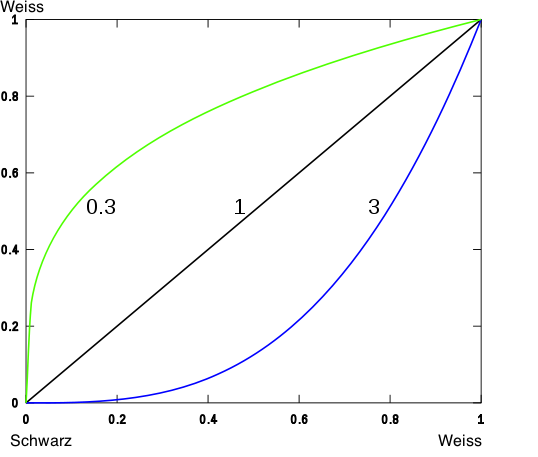
\includegraphics[width=0.5\textwidth]{figure/gamma-korrektur}\\

\textbf{Fall 1:} Ein $\gamma=1/2.2$ encodiertes Bild bedeutet, dass dunklere Pixel einen h�heren Helligkeitswert erhalten. Die Kodierung wird verwendet, um eine Ann�herung an die Wahrnehmung unserers Auges zu erreichen, welches dunkle Abstufungen besser wahrnimmt als helle.
Ist die Anzeige nun linear, werden diese Grauwerte auch so dargestellt, d.h. dunkle Grauwerte werden heller. Das Gesamtgamma des Systems entspricht $\gamma=1/2.2$\\
Rohbild (ohne Encoding): 

\includegraphics[width=\textwidth]{figure/gamma-linear}\\

Helleres Bild:

\includegraphics[width=\textwidth]{figure/gamma-0_45}


\textbf{Fall 2:} Bild Gamma encodiert, Anzeige f�hrt Gamma Korrektur durch. Das Gesamtgamma des Systems entspricht $\gamma=1$, d.h. die Gamma Kodierung wird bei der Anzeige korrigiert indem hellere Grauwerte der Gammakurve entsprechend dunkler dargestellt werden.\\ 
Rohbild (ohne Encoding)==Dargestelltes Bild: 

\includegraphics[width=\textwidth]{figure/gamma-linear}

\textbf{Fall 3:} Bild nicht Gamma encodiert, Anzeige ist Gamma korrigierend. Das Gesamtgamma des Systems entspricht $\gamma=2.2$\\
Rohbild (ohne Encoding): 

\includegraphics[width=\textwidth]{figure/gamma-linear}
Die dunklen Bereiche werden bei der Anzeige nochmals dunkler dargestellt.\\
Dargestelltes Bild:

\includegraphics[width=\textwidth]{figure/gamma-2_2}

 
\textbf{Fall 4:} Bild nicht Gamma encodiert, Anzeige f�hrt keine Gamma Korrektur durch. Das Gesamtgamma des Systems entspricht $\gamma=1$\\
Rohbild (ohne Encoding)==Dargestelltes Bild: 

\includegraphics{figure/gamma-linear}
}
\end{exercise}

